\section{测试数据}


\subsection{测试数据概述}
系统中的数据存储结构清晰,各表之间关系合理,主要包含以下数据表:

\begin{itemize}
    \item \textbf{原始数据表}:
    \begin{itemize}
        \item raw\_recruitment\_boss:存储BOSS直聘平台的原始招聘数据,容量56 MB,包含18,290条记录
        \item raw\_recruitment\_liepin:存储猎聘网的原始招聘数据,容量304 kB,包含220条记录
    \end{itemize}
    
    \item \textbf{核心业务表}:
    \begin{itemize}
        \item jobs:职位信息表,容量9,384 kB,包含18,166条记录
        \item recruitment\_mv:招聘信息物化视图,容量8,432 kB,包含18,166条记录
        \item companies:公司信息表,容量2,504 kB,包含8,691条记录
    \end{itemize}
    
    \item \textbf{地址相关表}:
    \begin{itemize}
        \item job\_address:职位地址关联表,容量1,240 kB,包含18,166条记录
        \item company\_address:公司地址关联表,容量784 kB,包含10,205条记录
        \item addresses:标准化地址表,容量256 kB,包含329条记录
    \end{itemize}

\end{itemize}


从数据规模来看,系统主要以BOSS直聘数据为主,辅以少量猎聘网数据。数据表之间的记录数量关系合理,反映了正确的业务关联。例如,一个职位对应一条地址记录(job\_address与jobs记录数相同),而一个公司可能有多个地址(company\_address记录数大于companies)。系统整体数据质量良好,表结构设计合理,为应用功能提供了可靠的数据基础。

\subsection{界面展示}

\subsubsection{MapPage 地图页面}
如图\ref{fig:map_page}所示,MapPage是一个专注于地理数据可视化的界面,其核心功能是展示各地区的薪资分布情况。同时提供区域薪资水平和热力图两种不同的地图视图模式,让用户能够直观且全面地了解不同地区的薪资水平分布状况。


\begin{figure}[htbp]
    \centering
    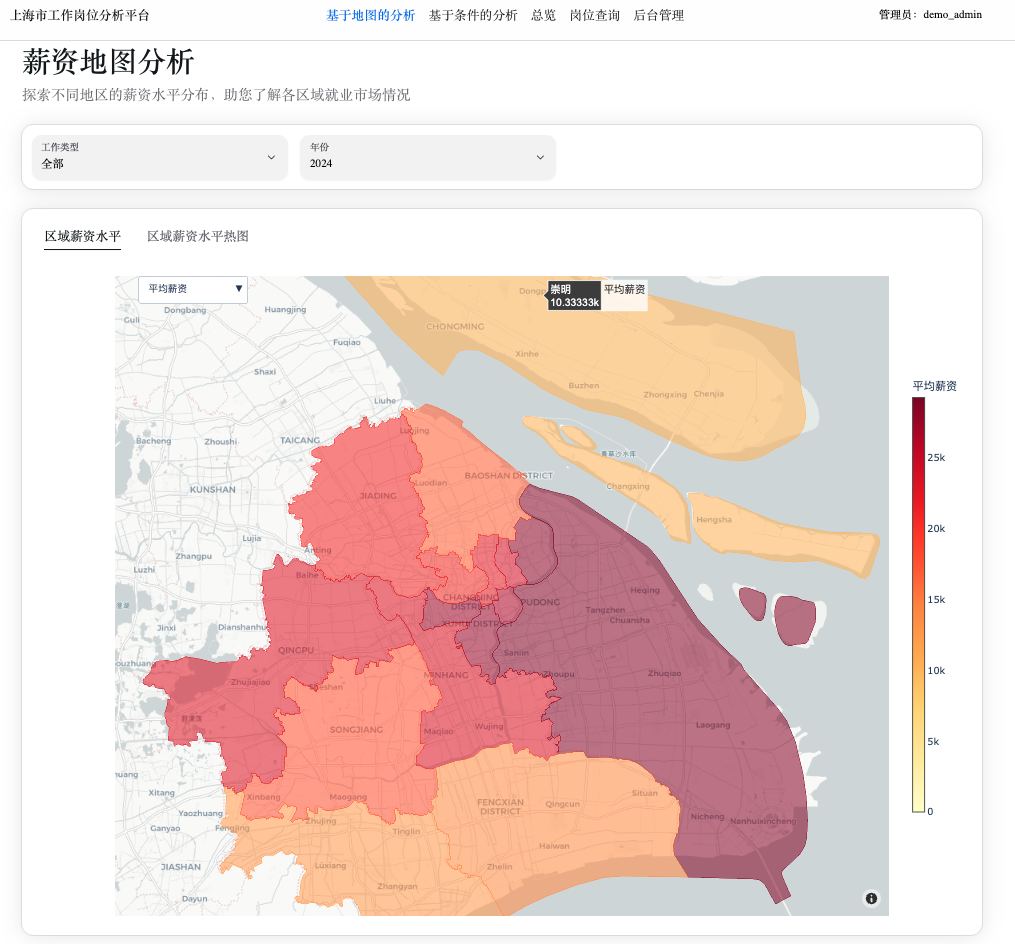
\includegraphics[width=1.0\textwidth]{figures/map_page.png}
    \caption{地图页面}
    \label{fig:map_page}
\end{figure}

\begin{figure}[htbp]
    \centering
    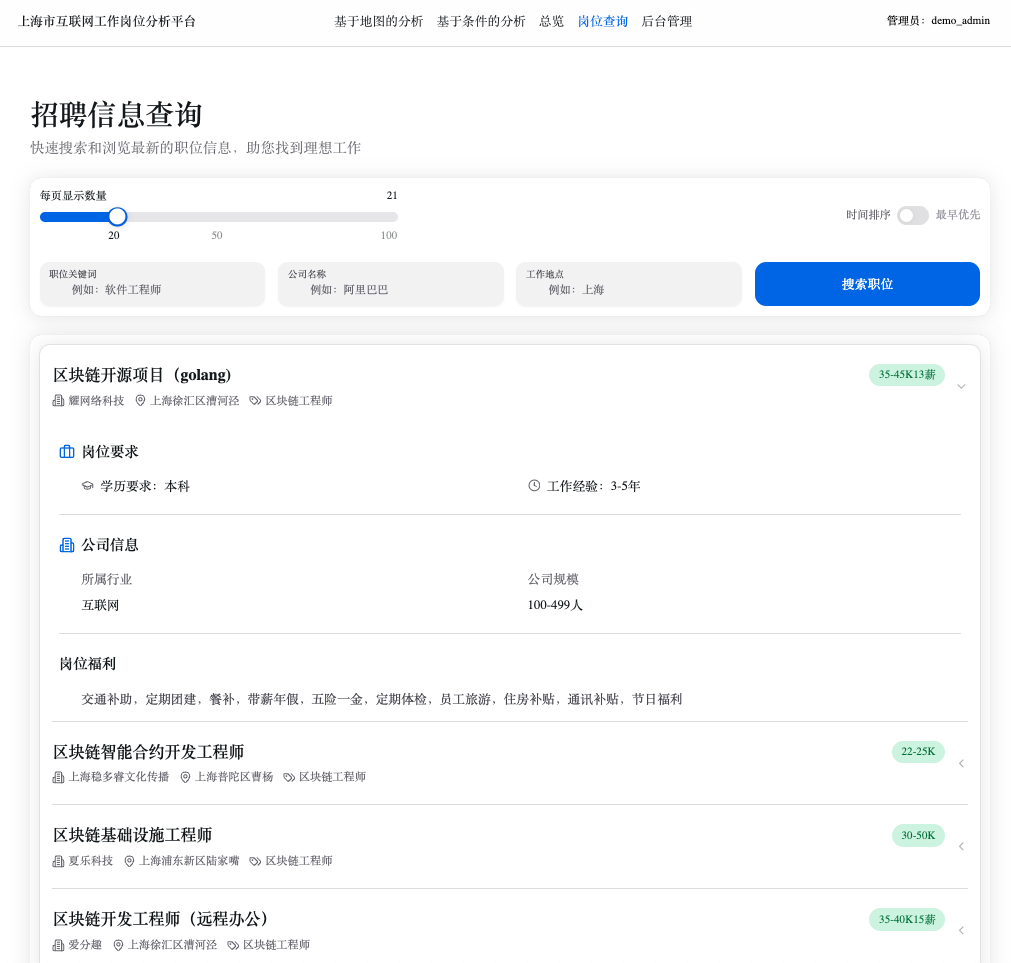
\includegraphics[width=1.0\textwidth]{figures/recruitment_page.png}
    \caption{招聘信息页面}
    \label{fig:recruitment_page}
\end{figure}

\begin{figure}[htbp]
    \centering
    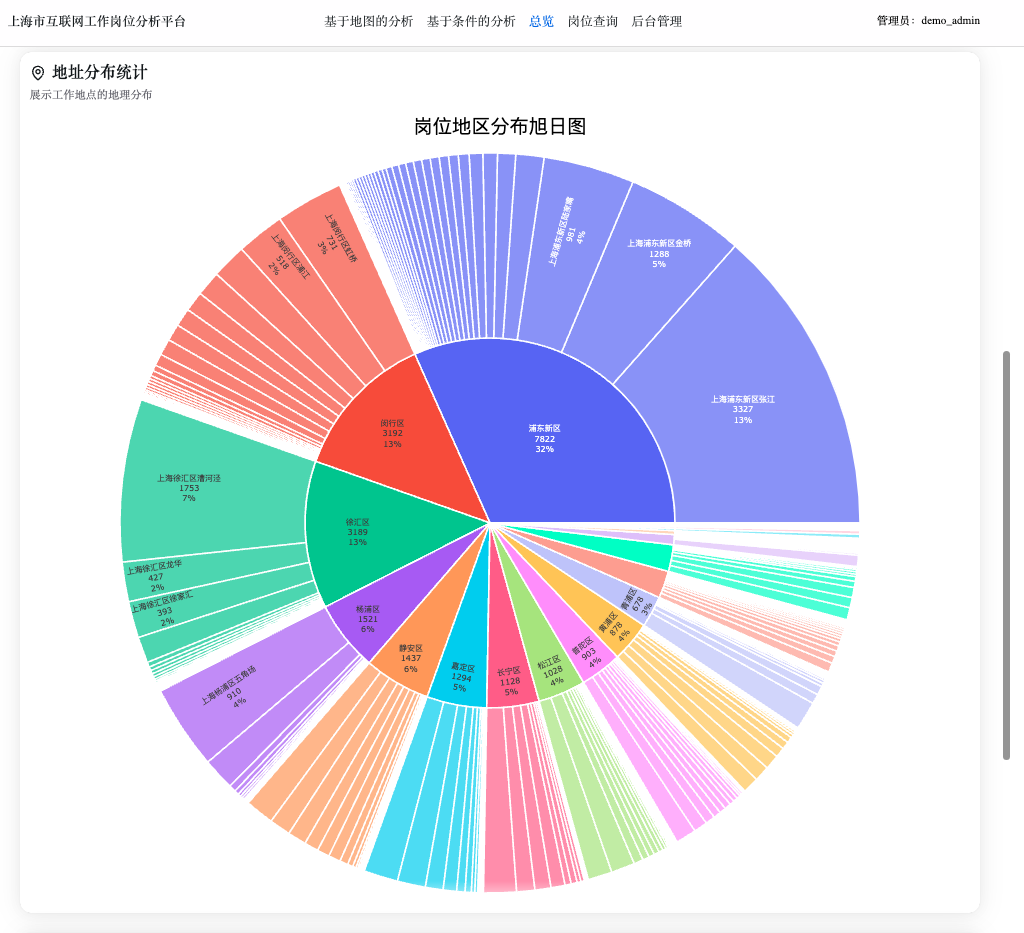
\includegraphics[width=1.0\textwidth]{figures/overview_page.png}
    \caption{概览页面}
    \label{fig:overview_page}
\end{figure}

\begin{figure}[htbp]
    \centering
    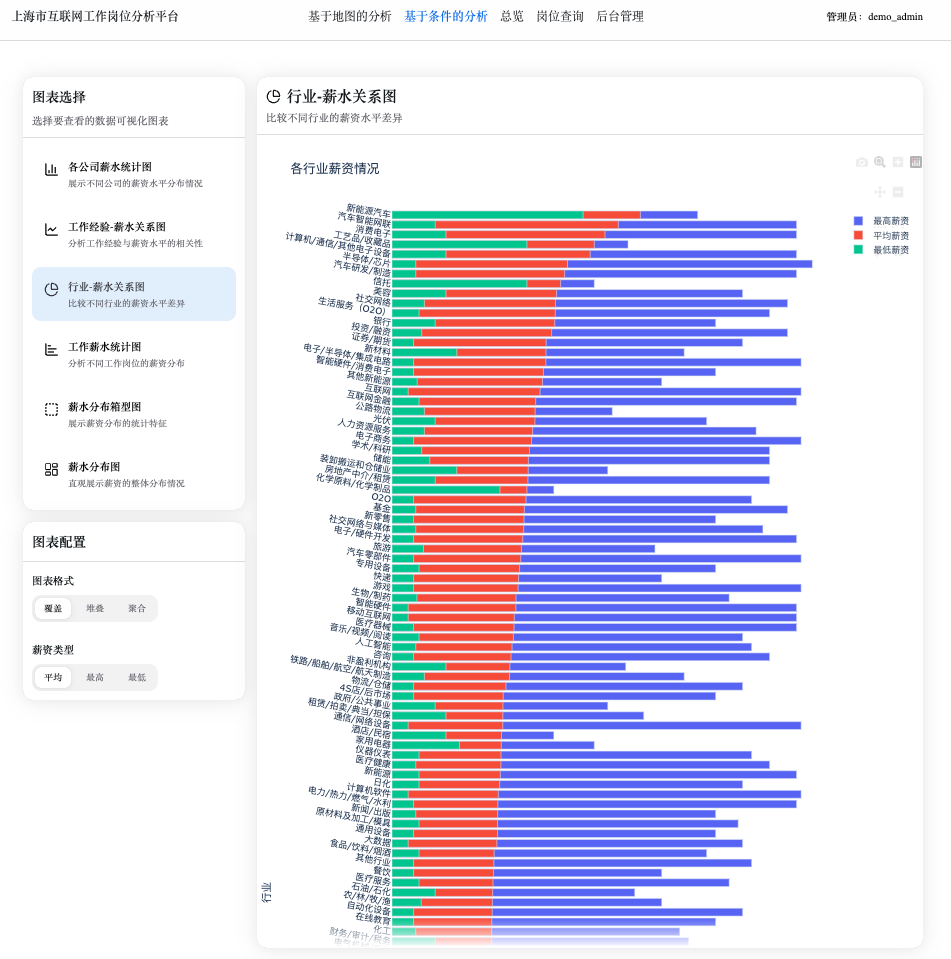
\includegraphics[width=1.0\textwidth]{figures/filter_page.png}
    \caption{筛选分析页面}
    \label{fig:filter_page}
\end{figure}

\begin{figure}[htbp]
    \centering
    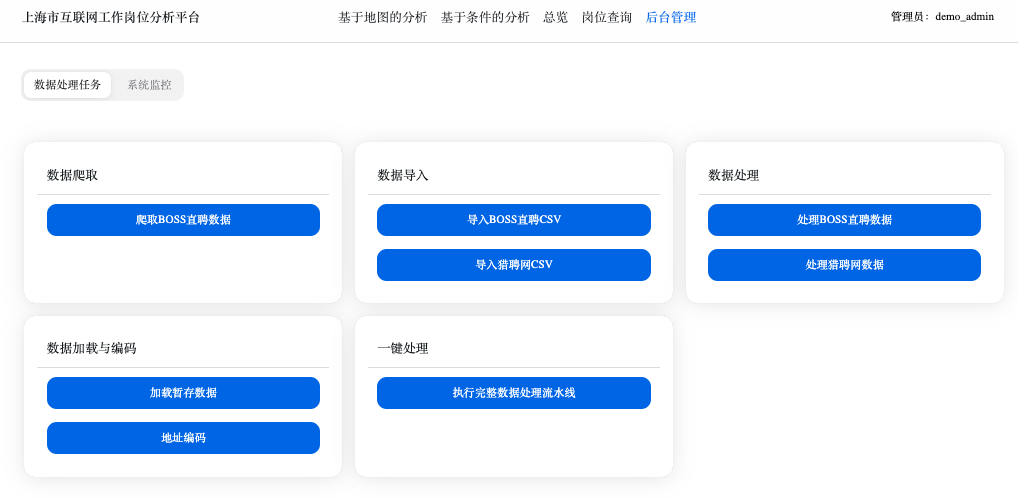
\includegraphics[width=1.0\textwidth]{figures/task_page1.png}
    \caption{任务管理页面}
    \label{fig:task_page_1}
\end{figure}

\begin{figure}[htbp]
    \centering
    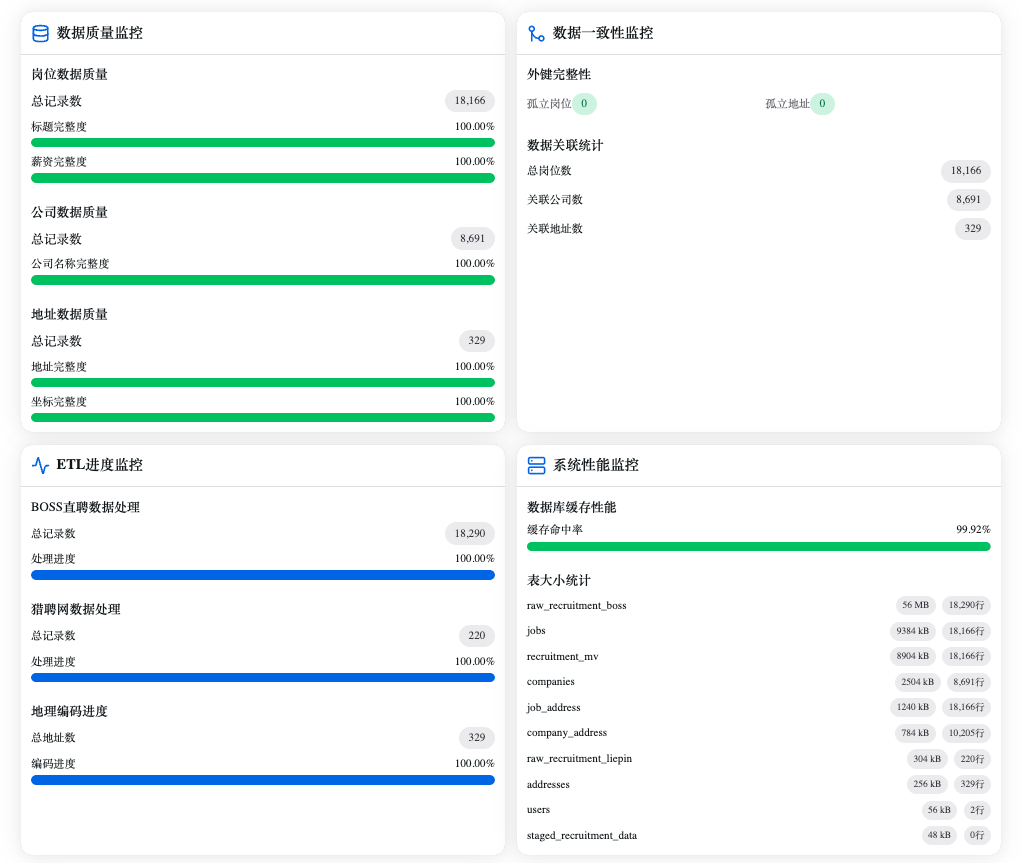
\includegraphics[width=1.0\textwidth]{figures/task_page2.png}
    \caption{系统监控页面}
    \label{fig:task_page_2}
\end{figure}


\subsubsection{RecruitmentPage 招聘信息页面}
如图\ref{fig:recruitment_page}所示,RecruitmentPage是一个功能完备的招聘信息查询平台,为用户提供精确的职位搜索体验。用户可以通过输入职位关键词、公司名称和工作地点等条件进行精确搜索,并可以灵活调整每页显示的信息数量(范围从1到100条)以及选择按时间的排序方式(最新或最早优先)。所有招聘信息都以清晰的卡片形式呈现,每张卡片都包含详尽的公司信息、具体的岗位要求以及完整的福利待遇说明。

\subsection{OverviewPage 概览页面}
如图\ref{fig:overview_page}所示,OverviewPage作为数据总览平台,通过丰富的数据可视化图表全方位展示就业市场概况。页面集中呈现了职位分布、地址分布、教育经验分布等多个维度的统计信息,并配备了直观的滑块控件,允许用户自由调整显示的职位数量(范围从1到200个),帮助用户快速准确地把握当前就业市场的整体态势。

\subsubsection{FilterPage 筛选分析页面}
如图\ref{fig:filter_page}所示,FilterPage是为用户提供深度的数据洞察能力。页面整合了多种专业的数据可视化图表,包括详细的公司薪资统计、经验与薪资的关系分析、行业薪资分布等核心指标。用户可以根据需求选择不同的图表类型,并通过调整展示模式(覆盖、堆叠或聚合)、薪资类型(平均值、最高值或最低值)以及学历条件等参数,进行全方位的数据分析。

\subsection{TaskPage 任务管理页面}
如图\ref{fig:task_page_1}所示,TaskPage的数据处理任务是一个面向管理员的专业数据处理任务管理平台,提供全面的数据管理功能。界面采用直观的卡片式布局,系统地组织各类数据任务,包括BOSS直聘平台的数据爬取、BOSS直聘和猎聘网的数据导入、数据处理以及地址编码等核心功能。特别设计了一键式操作选项,支持执行完整的数据处理流水线,大大提高了数据管理的效率和便捷性。

如图\ref{fig:task_page_2}所示,系统监控页面全面展示了数据处理和存储的运行状况:在数据质量方面,系统共处理了18,284条岗位数据、8,689条公司数据和330条地址数据,各项数据的完整度均达到100\%;在数据一致性方面,系统中没有出现孤立的岗位和地址记录,确保了数据的关联完整性;在ETL处理方面,BOSS直聘的18,290条数据和猎聘网的220条数据均已完成处理,地理编码任务也已全部完成;在系统性能方面,数据库存储使用率达到99.91\%,各数据表大小合理分布,从raw\_recruitment\_boss表的56MB到users表的56KB不等,整体运行状态良好。



